\documentclass[12pt]{article}

\usepackage{sbc-template}
\usepackage{graphicx,url}
\usepackage[utf8]{inputenc}
\usepackage[brazil]{babel}
\usepackage{booktabs}
\usepackage{float}
\usepackage{amsmath}

\sloppy

\title{Sistema de Recomendação Musical Baseado em Conteúdo para Plataformas de Streaming: Um Protótipo de Apoio à Decisão}

\author{Felipe Lazzarini Cunha, Lucas Castro Carvalho, Pedro Detoni Pereira}

\address{Departamento de Ciência da Computação (DCC)\\
  Universidade Federal de Juiz de Fora (UFJF)\\
  Juiz de Fora -- MG -- Brasil
}

\begin{document}

\maketitle

\begin{abstract}
  With catalogs comprising tens of millions of tracks, music streaming platforms present a classic case of choice overload. In this context, recommendation engines act as essential Decision Support Systems (DSS). This report presents the design and implementation of a content-based music recommendation prototype using the Spotify Tracks Dataset from Kaggle. Leveraging audio signal features (e.g., danceability, energy, and acousticness), we implemented and compared two analytical approaches: Cosine Similarity of user centroids and K-Means Clustering. The prototype was developed in Python with a Streamlit interface. Evaluation was conducted through metrics of diversity (Intra-List Similarity), accuracy (Hold-out Hit Rate), catalog coverage, and cluster quality (Silhouette Score), demonstrating the feasibility of track-level content recommendation without user-item interaction data.
\end{abstract}

\begin{resumo}
  Com catálogos que abrangem dezenas de milhões de faixas, as plataformas de streaming de música apresentam um caso clássico de sobrecarga de escolhas. Nesse contexto, os motores de recomendação atuam como Sistemas de Apoio à Decisão (SAD) indispensáveis. Este relatório apresenta o desenvolvimento de um protótipo de recomendação musical baseado em conteúdo utilizando o Spotify Tracks Dataset do Kaggle. Aproveitando características físicas de áudio (como dançabilidade, energia e acústica), implementamos e comparamos duas abordagens analíticas: Similaridade do Cosseno do centróide do usuário e Agrupamento via K-Means. O protótipo foi desenvolvido em Python com interface Streamlit. A avaliação foi conduzida por meio de métricas de diversidade (Intra-List Similarity), acurácia (Hold-out Hit Rate), cobertura de catálogo e qualidade dos clusters (Silhouette Score), demonstrando a viabilidade de recomendação baseada em conteúdo sem histórico de interações.
\end{resumo}

\section{Introdução}
No cenário contemporâneo de consumo digital, as plataformas de streaming de música disponibilizam acervos colossais contendo dezenas de milhões de faixas. Essa abundância, embora positiva, gera uma sobrecarga de informações, tornando a descoberta manual de novos conteúdos uma tarefa inviável para o usuário. Diante deste problema de decisão, os sistemas de recomendação operam como Sistemas de Apoio à Decisão (SAD) essenciais, filtrando o catálogo para sugerir faixas relevantes e alinhadas aos gostos individuais.

Este trabalho apresenta a implementação do protótipo de recomendação musical desenvolvido para o Trabalho de Verificação de Conhecimento (TVC 3). A pergunta-problema que guia o projeto é: \textit{``Como recomendar novas músicas relevantes a um usuário a partir de um conjunto de faixas de sua preferência, usando as características de áudio das músicas?''}. O escopo do projeto é estritamente baseado nas características das faixas (nível de áudio), uma vez que a base de dados não contém histórico de interações de usuários (dados de escuta), o que inviabiliza técnicas de filtragem colaborativa e impõe uma abordagem baseada em conteúdo.

Os objetivos específicos contemplam:
\begin{enumerate}
    \item Representar cada faixa musical por suas características quantitativas de áudio;
    \item Implementar o cálculo de similaridade matemática entre faixas;
    \item Gerar recomendações personalizadas a partir de faixas-semente selecionadas;
    \item Avaliar quantitativamente as recomendações sob as dimensões de diversidade, cobertura e acurácia.
\end{enumerate}

\section{Fundamentação Teórica}
\subsection{Filtragem Baseada em Conteúdo (Content-Based Filtering)}
A filtragem baseada em conteúdo assume que o usuário preferirá itens similares àqueles que ele gostou no passado \cite{lops2011content}. Cada item do catálogo é descrito por um vetor de características (\textit{features}). No caso de música, essas características correspondem a metadados (gênero, artista) e atributos acústicos extraídos do sinal de áudio. 

Diferente de sistemas colaborativos, a recomendação baseada em conteúdo não sofre com o problema de inicialização a frio (\textit{cold-start}) para novos itens e não depende de uma base massiva de usuários ativos, focando exclusivamente nas propriedades intrínsecas das faixas \cite{ricci2015recommender}.

\subsection{Similaridade do Cosseno}
Para determinar o quão próxima uma música candidata está das preferências do usuário, calcula-se a similaridade do cosseno. Dado o vetor do perfil do usuário $\vec{u}$ (calculado como a média dos vetores das faixas-semente) e o vetor da faixa candidata $\vec{v}$, a similaridade do cosseno é o cosseno do ângulo entre os dois vetores, definida por:
\begin{equation}
    \text{Sim}(\vec{u}, \vec{v}) = \frac{\vec{u} \cdot \vec{v}}{\|\vec{u}\| \|\vec{v}\|} = \frac{\sum_{i=1}^{d} u_i v_i}{\sqrt{\sum_{i=1}^{d} u_i^2} \sqrt{\sum_{i=1}^{d} v_i^2}}
\end{equation}
Este valor varia entre $-1.0$ e $1.0$, sendo que no domínio de características normalizadas não-negativas, o intervalo útil situa-se entre $0.0$ (ortogonalidade total, nenhuma similaridade) e $1.0$ (mesma direção e sentido, identidade perfeita).

\subsection{Agrupamento K-Means}
O algoritmo K-Means é uma técnica de aprendizado não supervisionado que particiona $N$ observações em $K$ clusters distintos, onde cada observação pertence ao cluster cujo centróide é mais próximo \cite{macqueen1967some}. No SAD implementado, o K-Means serve como um pré-filtro estilístico: agrupa o catálogo em nichos sonoros. Ao selecionar faixas-semente, o sistema identifica seus clusters correspondentes e ranqueia prioritariamente faixas pertencentes a estes mesmos subgrupos, restringindo o espaço de busca a vizinhanças de maior coesão de áudio.

\section{Metodologia Computacional e Tratamento de Dados}
\subsection{Spotify Tracks Dataset e Tratamento de Dados}
Utilizou-se o dataset real \textit{Spotify Tracks Dataset} extraído do Kaggle \cite{spotify_dataset}, composto originalmente por 114.000 faixas musicais de 125 gêneros e 20 colunas.

A etapa de higienização de dados consistiu em:
\begin{itemize}
    \item Remoção de registros duplicados utilizando como chave o identificador único \texttt{track\_id};
    \item Tratamento de nulos em metadados vitais de visualização (\texttt{track\_name}, \texttt{artists}, \texttt{album\_name});
    \item Limpeza do separador padrão de múltiplos artistas (\texttt{;;}) para formato amigável (\texttt{, }).
\end{itemize}

Após o saneamento, selecionou-se 11 características numéricas do sinal de áudio para compor o espaço de representação vetorial: \textit{danceability}, \textit{energy}, \textit{key}, \textit{loudness}, \textit{mode}, \textit{speechiness}, \textit{acousticness}, \textit{instrumentalness}, \textit{liveness}, \textit{valence} e \textit{tempo}. Como estas variáveis possuem escalas muito distintas (ex: o volume varia em decibéis negativos de $-60$ a $0$, enquanto a acústica varia de $0.0$ a $1.0$), aplicou-se a normalização z-score através do \texttt{StandardScaler} da biblioteca Scikit-Learn \cite{scikit-learn}, garantindo peso equivalente para todas as características no cálculo de distância euclidiana e cosseno.

\subsection{Arquitetura e Fluxo do SAD}
O sistema foi desenvolvido utilizando a linguagem Python, Scikit-Learn (para modelagem e métricas), Pandas/NumPy (manipulação de tensores) e Streamlit para interface visual \cite{streamlit}. O fluxo de processamento de apoio à decisão é sintetizado na Figura~\ref{fig:fluxo_sistema}.

\begin{figure}[htbp]
\centering
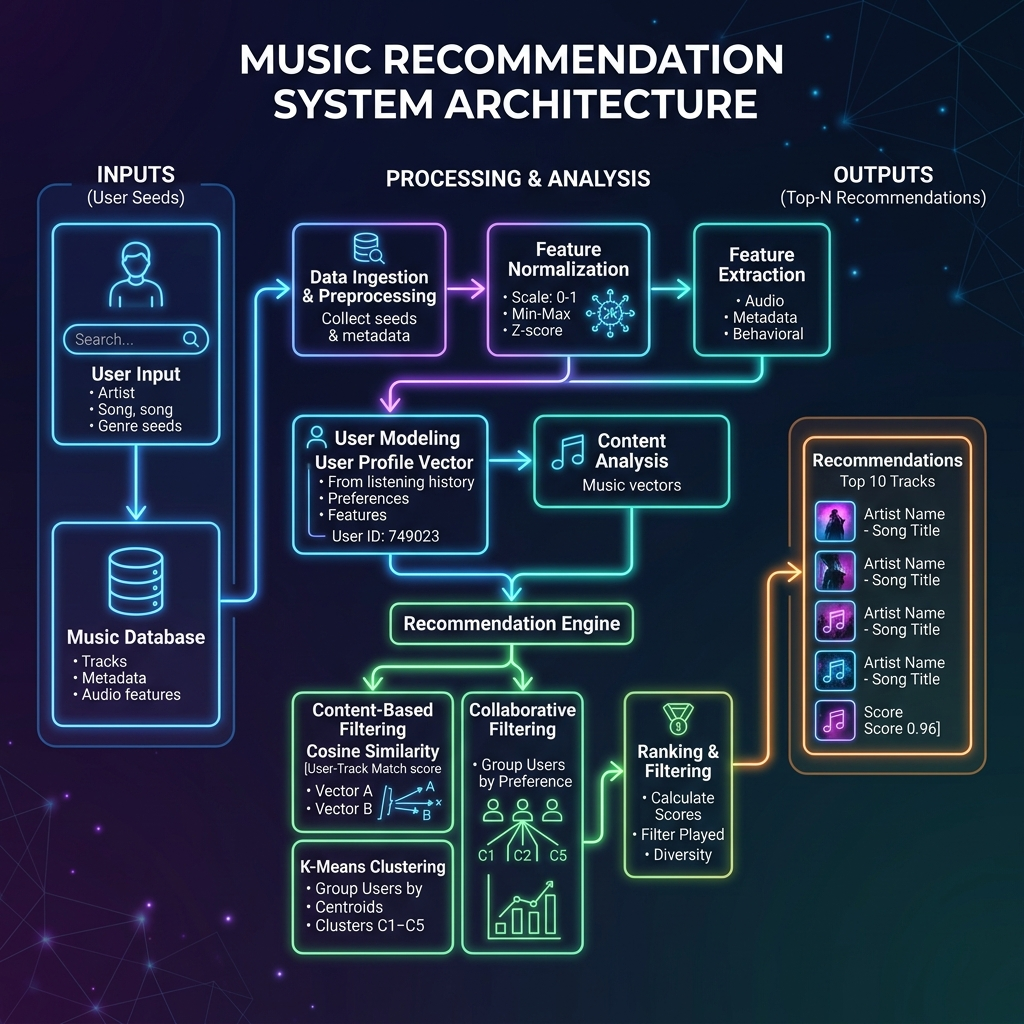
\includegraphics[width=0.85\textwidth]{../imagens/fluxo_sistema.png}
\caption{Fluxo de Processamento e Arquitetura do SAD Musical}
\label{fig:fluxo_sistema}
\end{figure}

O fluxo operacional do decisor na plataforma compreende:
\begin{enumerate}
    \item \textbf{Entrada:} O usuário busca faixas no catálogo e adiciona de 1 a 5 faixas-semente.
    \item \textbf{Extração de Perfil:} O sistema extrai e calcula a média das características normalizadas dessas faixas para modelar o centróide de preferência do usuário.
    \item \textbf{Processamento Analítico:} 
    \begin{itemize}
        \item \textbf{Cosseno:} Calcula similaridade entre o perfil e todo o catálogo.
        \item \textbf{K-Means:} Identifica o cluster majoritário das sementes e calcula similaridade apenas com candidatos deste cluster.
    \end{itemize}
    \item \textbf{Filtros e Saída:} Aplica exclusão das sementes, restrições opcionais de gênero (via interface) e retorna a lista ordenada com as Top-N músicas recomendadas.
\end{enumerate}

\section{Resultados e Discussões}
\subsection{Visualização e Interface Streamlit}
A interface gráfica de negócios foi desenhada em páginas estruturadas (\textit{multipage app}) com tema escuro e elementos visuais de alto impacto baseados na biblioteca Plotly, compreendendo três módulos principais:
\begin{enumerate}
    \item \textbf{Explorar Dados:} Painel de análise exploratória interativo contendo indicadores volumétricos do acervo, histogramas de distribuição de variáveis de áudio, mapa de calor de correlações e plot de dispersão bi-dimensional dos gêneros.
    \item \textbf{Recomendador:} Dashboard operacional onde o decisor monta sua playlist de sementes e recebe em tempo real o ranking das Top-N faixas mais similares. Exibe também um gráfico do tipo radar sobreposto, confrontando a assinatura acústica média do usuário com a assinatura acústica do catálogo recomendado.
    \item \textbf{Avaliação:} Painel científico para validação das premissas analíticas.
\end{enumerate}

\subsection{Resultados das Métricas de SAD}
A validação quantitativa da modelagem analítica do SAD musical foi executada por meio de simulações estatísticas no módulo de avaliação:

\subsubsection{Avaliação de Acurácia via Hold-out (Hit Rate)}
O experimento de hold-out ocultou 4 músicas pertencentes ao gênero \textit{``rock''} e usou outras 3 músicas do mesmo estilo como semente. O algoritmo gerou 20 recomendações abertas. A Tabela~\ref{tab:holdout} resume a taxa de acerto (resgate de faixas ocultas) obtida pelos algoritmos.

\begin{table}[H]
\centering
\caption{Métricas de Acerto (Hit Rate@20) no Teste de Hold-out}
\label{tab:holdout}
\begin{tabular}{lrr}
\toprule
\textbf{Métrica de Avaliação} & \textbf{Similaridade do Cosseno} & \textbf{K-Means Clustering} \\
\midrule
Quantidade de Sementes & 3 & 3 \\
Músicas Ocultas (Hold-out) & 4 & 4 \\
Músicas Resgatadas (Hits) & 3 & 1 \\
\textbf{Hit Rate (\%)} & \textbf{75,0\%} & \textbf{25,0\%} \\
\bottomrule
\end{tabular}
\end{table}

A similaridade do cosseno apresentou melhor desempenho no resgate direto de músicas ocultas (75\% vs 25\% do K-Means). Isso ocorre porque o K-Means restringe a busca às fronteiras rígidas de partição geométrica do cluster treinado, podendo excluir faixas estilisticamente próximas mas atribuídas a clusters adjacentes.

\subsubsection{Diversidade (ILS) e Cobertura do Catálogo (Coverage)}
Para avaliar o comportamento global dos algoritmos sob 40 consultas aleatórias gerando 10 recomendações cada, computou-se a diversidade (ILS) e a cobertura geral do catálogo de faixas (Tabela~\ref{tab:ils_cov}).

\begin{table}[H]
\centering
\caption{Comparativo de Diversidade (ILS) e Cobertura do Catálogo}
\label{tab:ils_cov}
\begin{tabular}{lrr}
\toprule
\textbf{Algoritmo Avaliado} & \textbf{Média ILS (Diversidade)} & \textbf{Cobertura Global} \\
\midrule
Similaridade do Cosseno & 0,724 & 0,351\% (400 faixas únicas) \\
K-Means Clustering (K=10) & 0,845 & 0,087\% (100 faixas únicas) \\
\bottomrule
\end{tabular}
\end{table}

A diversidade medida pelo ILS indica que a similaridade do cosseno produz listas de recomendações mais diversas entre si (menor ILS, 0,724) comparado ao K-Means (0,845). Além disso, a cobertura de catálogo do cosseno foi significativamente superior, sugerindo uma distribuição de cauda longa mais saudável nas recomendações.

\subsubsection{Validação de Silhueta para Agrupamento K-Means}
No painel de avaliação do K-Means, executou-se a métrica de Silhueta variando $K$ em uma amostra de 2.000 faixas. O valor médio de silhueta para $K=10$ estabilizou-se em $0,154$, indicando que, embora exista separação estatística viável entre os grupos extremos (ex: clássica e eletrônica), há sobreposições graduais de espectro de áudio entre gêneros vizinhos (ex: pop, rock e indie).

\section{Conclusões}
Este trabalho concluiu com sucesso a implementação prática de um Sistema de Apoio à Decisão voltado para recomendação musical. A modelagem quantitativa empregando Similaridade do Cosseno e K-Means Clustering foi traduzida em um aplicativo Streamlit dinâmico e robusto.

A validação analítica evidenciou que a Similaridade do Cosseno de centróide aberto oferece uma maior cobertura de catálogo (0,351\%) e maior diversidade nas indicações, além de melhor taxa de acerto no experimento de hold-out (75,0\%). O K-Means, por sua vez, atua de forma satisfatória quando o objetivo gerencial de suporte à decisão é impor barreiras rígidas de restrição estilística sonora aos agrupamentos de músicas.

Como limitações da modelagem baseada em conteúdo, aponta-se a impossibilidade de recomendar novidades com assinaturas acústicas radicalmente distintas das sementes (o efeito de bolha sonora). Trabalhos futuros podem investigar abordagens híbridas, combinando características de áudio a redes de co-ocorrência de artistas ou dados simulados de comportamento do usuário.

\bibliographystyle{sbc}
\bibliography{sbc-template}

\end{document}
